Для начала проверим работоспособность адаптера, настроив его на нужное соединение. Это можно осуществить, просканировав сеть (рис.~\ref{mm_1:mm_1}) на доступные беспроводные соединения, выбрав необходимое и прописав настройки в файле /etc/network/interfaces (рис.~\ref{mm_2:mm_2} и~\ref{mm_3:mm_3}). В результате выполнения команды iwconfig (рис.~\ref{mm_4:mm_4}) можно увидеть, что уровень сигнала wlan0 нулевой, однако после перезаргузки системы командой reboot сеть работает в режиме по умолчанию --- managed (рис.~\ref{mm_5:mm_5}). 

\begin{figure}[h!]
\center{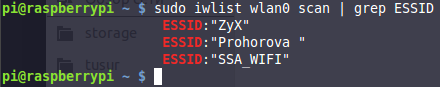
\includegraphics[width=0.6\linewidth]{mm_1}}
\caption{ Сканирование сети на доступные соединения }
\label{mm_1:mm_1}
\end{figure}


\begin{figure}[h!]
\center{
\includegraphics[width=0.6\linewidth]{mm_2}}
\caption{ Путь к config-фалу с настройками интерфейсов }
\label{mm_2:mm_2}
\end{figure}


\begin{figure}[h!]
\center{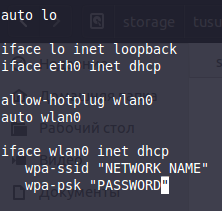
\includegraphics[width=0.3\linewidth]{mm_3}}
\caption{ Файл <<interfaces>> }
\label{mm_3:mm_3}
\end{figure}

\begin{figure}[h!]
\center{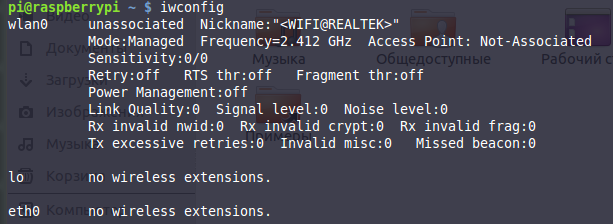
\includegraphics[width=0.7\linewidth]{mm_4}}
\caption{ Результат выполнения команды iwconfig }
\label{mm_4:mm_4}
\end{figure}

\begin{figure}[h!]
\center{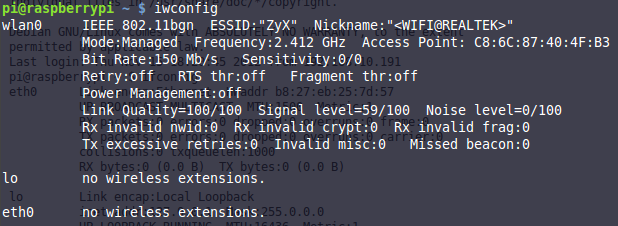
\includegraphics[width=0.7\linewidth]{mm_5}}
\caption{ Результат выполнения команды iwconfig после перезагрузки системы }
\label{mm_5:mm_5}
\end{figure}

Бесповодные сетевые адаптеры стандарта WNIC 802.11 могут поддерживать шесть рабочих режимов: master, managed,
ad-hoc, mesh, repeater и monitor. Режим монторинга пакетов (monitor mode) аналогичен смешанному режиму (promiscuous mode), однако применим только для беспроводных сетей. В отличии от смешанного режима, устройства не обязательно должны быть в сети. Режим мониторинга пакетов позволяет перехватывать все пакеты, которые могут быть распознаны WNIC-адаптером. Данный режим зависит от драйвера, архитектуры и чипсета устройства. Согласно этим ограничениям, не все адаптеры поддерживают monitor mode. При этом устройство может в определенный момент времени находиться только в одном режиме \cite{article}.

Настроим адаптер в режим мониторинга пакетов. Для этого необходимо ввести команду:

\begin{verbatim}
$ sudo iwconfig wlan0 mode monitor
\end{verbatim} 

При попытке ввести данную команду система выводит сообщение о том, что ресурс занят (рис.~\ref{mm_6:mm_6}).


\begin{figure}[h!]
\center{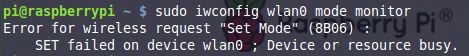
\includegraphics[width=0.6\linewidth]{mm_6}}
\caption{ Результат выполнения команды iwconfig }
\label{mm_6:mm_6}
\end{figure}

Это связано с тем, что в системе работает network interface plugging daemon~\cite{daemon} --- программа, работающая в системе в фоновом режиме и отвечающая за автоматическое подсоединеие сетевых интерфейсов. Эта же прорамма устанавливает для устройств режим по умолчанию. Необходимо ее отключить для того, чтобы перевести устройство в другой режим работы.

Напишем небольшой bash-скрипт, который будет переводить адаптер в режим перехвата пакетов и содержать следующие команды:

\begin{verbatim}
$ #!/bin/bash
$ sudo service ifplugd stop #останавливаем работу демона
$ sudo ifconfig wlan0 down #отключаем wi-fi соединение
$ sudo iwconfig wlan0 mode monitor #включаем прослушивающий режим
$ sudo ifconfig wlan0 up #включаем wi-fi соединение
$ sudo service ifplugd start #запускаем демона
$ iwconfig #проверям настройки
\end{verbatim} 

Результат работы скрипта приведен на рисунке~\ref{mm_7:mm_7}. Wi-Fi-адаптер теперь работает в режиме перехвата пакетов. Данный скрипт необходимо запускать снова при перезапуске системы.

\begin{figure}[h!]
\center{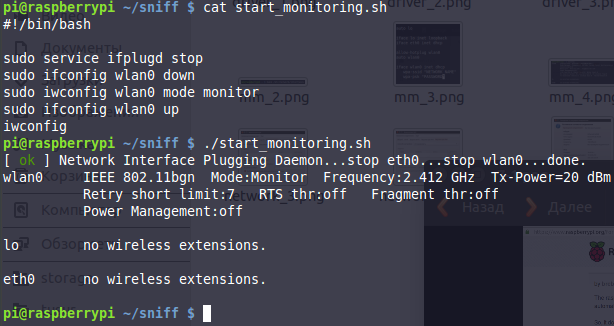
\includegraphics[width=0.8\linewidth]{mm_7}}
\caption{ Результат выполнения скрипта }
\label{mm_7:mm_7}
\end{figure}

\clearpage






